\documentclass[12pt]{article}
\usepackage{ulem}
\usepackage{apacite}
\usepackage{amsmath}
\usepackage{amssymb}
\usepackage{graphicx}
\usepackage{enumerate}
\usepackage{algorithm}
\usepackage{algorithmicx}
\usepackage{algpseudocode}
\usepackage{setspace}
\usepackage[rgb]{xcolor}
\usepackage[numbers]{natbib}
\usepackage[a4paper,margin=2cm]{geometry}
\usepackage[colorlinks=true, urlcolor=blue, linkcolor=blue, citecolor=blue]{hyperref}

\newtheorem{lemma}{Lemma}[section]
\newtheorem{theorem}{Theorem}[section]
\newtheorem{corollary}{Corollary}[section]
\newtheorem{definition}{Definition}[section]

\begin{document}
\begin{spacing}{1.15}
\title{\bf Final Project Report: The Hanabi Game}
\author{Xiuhan Wang, Jing Wei}
\date{\today}
\maketitle

\section{Introduction}
The Hanabi game is a benchmark challenge in fully cooperative games of imperfect information; it's very different from adversarial two-player zero-sum games which have been studied more\cite{bard2020the}. But non-zero-sum scenarios are more important in real life.

The Hanabi game was proved \textsf{NP}-hard even if all hidden information is revealed.\cite{baffier2017hanabi} The hand-coded mathematical ``hat guessing game'' strategy\cite{cox2015how} held state-of-the-art results from March 2016 until December 2019. In five-player games, it almost achieved the best performance resulted by a cheating strategy where each player sees his own cards and uses the information strategy. However, it performed badly in the two-player setting\cite{bouzy2017playing}; and it is not generalizable to similar games. A Monte-Carlo tree search algorithm is given by \cite{walton-rivers2017evaluating}; but the performance is still not very good.

Foerster and Song proposed a method of Bayesian action decoder (BAD)\cite{foerster2018bayesian}. The key idea is a joint public belief over players' private features to resolve recursive belief over beliefs, and sampling a deterministic partial policy to resolve the dilemma between informative actions and stochastic actions for exploration. BAD worked well in the two-player setting. Hu and Foerster continued to optimize BAD to SAD\cite{hu2020simplified} and incorperated search into SPARTA\cite{lerer2020improving} to achieve a new state-of-the-art result.

Then they come up with the method called ``other-play'' (OP)\cite{hu2020other} that work well on the zero-shot coordination scenario of the game. Previous studies on MARL usually focus on the self-play (SP) setting where agents are trained and tested both against with themselves, but agents naively trained by SP could do arbitrarily bad when paired with a partner they're not trained with. OP trains the agent with a copy of itself that is randomly permuted according to the symmetries in the game; hence it reduces the tendency towards arbitrary symmetry breaking. Agents trained with OP perform well when tested by cross-play, and also cooperate well with human.

This work is an improvement based on OP. Intuitively, the optimal strategies for symmetric games should be the same. As an analog, the convolutional neural network uses a symmetric network for training. We apply this idea to the network and reduce the network size by the symmetry group size.

\section{Rules for the Hanabi Game}

\textsl{Hanabi} is a game for two to five players. Each player holds four cards in his hand (or five if less than four players). Everyone can see all others' cards but not that of himself. Each card has a rank (1--5) and a color (red, green, blue, yellow or white). There are three 1s, two 2s, 3s, 4s and a 5 of each color; hence 50 cards in total. The players are fully cooperative---they want to play cards to build five stacks, one for each color, going consecutively from 1. The goal is to maximize the score, which is the total number of cards in the stack.

Players take turns to play. In one's turn, he must take exactly one of the following actions:

\begin{itemize}
\item \textbf{Hint.} To give a hint to others, the player chooses a color or a rank, then point out all cards matching that color or rank in another player's hand. Only ranks and colors that are present in the other player's hand can be chosen. To limit the number of hints, the group has initially eight information tokens and a token is consumed when giving a hint.
\item \textbf{Discard.} When there are less than eight information tokens, he can discard a card from his hand, draw a new card from the deck and recover an information token. The discarded card is visible to all players and the newly drawn card is visible only to all other players.
\item \textbf{Play.} The player can choose a card from his hand and try to put it in the stacks. It's successful if the rank is exactly one larger than the top of the stack corresponding to the color. If it's successful, put the card on the top of that stack. Recover one information token if there are less than eight and the rank played is 5. If the play is unsuccessful, discard the card and the group loses one life. When three lives are lost, the game ends immediately. Whether successful or not, the player draws a new card from the deck.
\end{itemize}

\begin{figure}[H]
\centerline{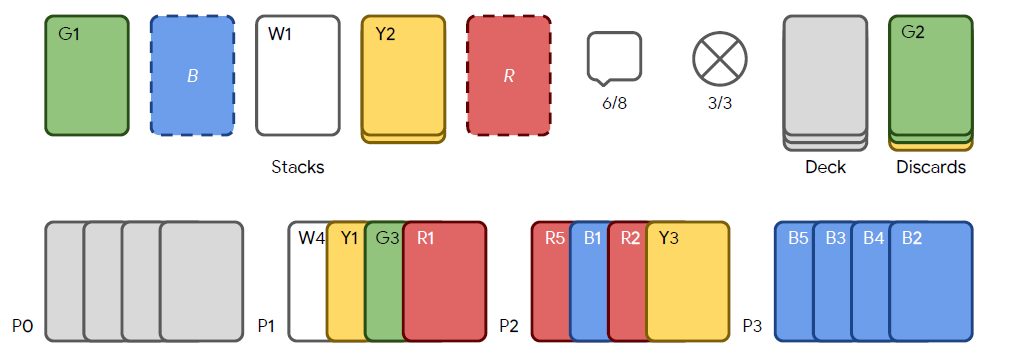
\includegraphics[width=6in]{fig1.png}}
\caption{An example of a four player Hanabi game from the point of view of player 0 (cite from \cite{bard2020the}).}
\label{Fig1}
\end{figure}

\section{Other-Play}
Let $\pi^1, \pi^2$ be the policies of the two players and let $J(\pi^1, \pi^2)$ be the reward. If the two players know each other, they can discuss the strategies and thus the goal is to find the optimal \[\pi^* = \arg \max_{\pi} J(\pi^1, \pi^2).\]

However, in real-world scenarios, the players don't know each other and can't discuss their strategies. Consider the following \textsl{lever coordination game}: two players, who don't know each other, will choose two levers independently. If the levers chosen are the same, they can get the reward of the lever. Otherwise, the reward is $0$. In Figure \ref{Fig2} (a), since they don't know each other, the optimal strategy is to pick one lever randomly, with expected reward $0.1$. However, in (b), the $1$-levers are still undistinguishable but there appears to be a $0.9$-lever. If they both take some $1$-lever, the expected reward is $0.11$. However, if they both take the $0.9$-lever, the reward is $0.9$, which is larger.

\begin{figure}[H]
\centerline{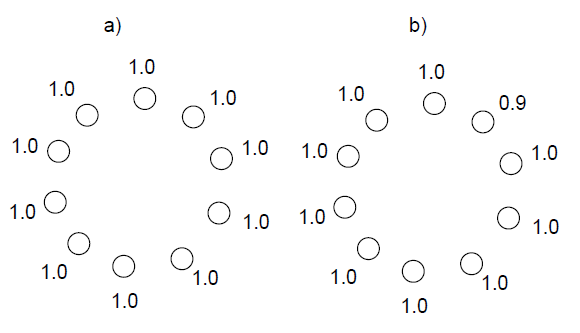
\includegraphics[width=4in]{fig2.png}}
\caption{An example of a lever coordination game (cite from \cite{hu2020other}).}
\label{Fig2}
\end{figure}

Similar scenarios also happen in our training. In the Hanabi game, the colors are symmetric and thus undistinguishable. For example, if two players know each other, they can use strategies like: ``If one player hints yellow, the other player should discard; If one player hints blue, the other player should play.'' If we change the roles of ``blue'' and ``yellow'', the new strategy behaves as good as the original one. However, if the two players don't know each other, one player may use the first strategy while the other uses the second one, which makes performance bad.

The key point is the players can't distinguish symmetric settings. Let $\Phi$ be the symmetric group, where each $\phi\in \Phi$ if after applying $\phi$ to the states and actions, the transitions, rewards and observations don't change. To break symmetries, the OP setting tries to find the optimal \[\pi^* = \arg \max_{\pi} \mathbb{E}_{\phi\sim \Phi} J(\pi^1, \phi(\pi^2))\] instead. In practice, while training a agent with policy $\pi$, we select a randomly permutation $\phi\in \Phi$ and let $\pi$ play with $\phi(\pi)$.

\section{Symmetric Networks}
Recall the convolutional neural networks, which uses symmetries to reduce the number of network parameters. The symmetries in the convolutional layer are translations. As an analog, since there are also symmetries in the Hanabi game, we can use a symmetric network to reduce the number of parameters. Precisely, let $\Phi = S_5$ be the symmetric group in the Hanabi game, and our network should satisfy:

\begin{itemize}
\item For every neuron $h$ in the network, there should also be neurons $\phi(h)$ for all $\phi\in \Phi$.
\item $h$ and $\phi(h)$ should have the same bias. If $h$ takes its input from a neuron $g$ with weight $\alpha$, then $\phi(h)$ takes input from $\phi(g)$ with the same weight.
\end{itemize}

In other words, the neurons are divided into equivalence classes $\{\phi(h)\mid \phi \in \Phi\}$ where they share a same set of weights and bias. Each equivalence classes has size at most $|\Phi|$. The way of constructing a network applies to various types of neurons including LSTM cells.

The symmetric network reduces the number of parameter by a factor about $|\Phi|$. In this specific problem, the Hanabi game, the network size becomes about $1 / 120$ from any original training method.

\section{Empirical Results}

\section{Conclusion}

\normalem
\bibliographystyle{apacite}
\bibliography{papers}
\end{spacing}
\end{document}
